\documentclass[10pt,a4paper]{article}
%\usepackage[natbibapa]{apacite} 
\usepackage{enumitem}
\usepackage{amsmath}
\usepackage{tikz}
\usepackage{physics}
\usetikzlibrary{automata,positioning}
%\bibliographystyle{apacite}

\usetikzlibrary{shapes.misc}
\usetikzlibrary{decorations.pathreplacing}

\title{Natural Language Processing (COS4861)}
\author{Adriaan Louw (53031377)}


\tikzset{basic/.style={draw,fill=blue!50!green!20,
                       text badly centered,minimum width=3em}}
\tikzset{input/.style={basic,circle}}
\tikzset{weights/.style={basic,rectangle,minimum width=2em}}
\tikzset{functions/.style={basic,circle,fill=blue!50!green!20}}
\newcommand{\addsymbol}{\draw[thick] (0.5em,0.5em) -- (0,0.5em) -- 
                        (0,-0.5em) --  (-0.5em,-0.5em)
                        (0em,0.75em) -- (0em,-0.75em)
                        (0.75em,0em) -- (-0.75em,0em);}
                        
\begin{document}

\maketitle

\section{Question 1}
\begin{enumerate}[leftmargin=\labelsep]
\item[1.1]
\end{enumerate}

\section{Question 2}
For $V_2(1):$

\begin{equation}
\begin{split}
V_1(1)P(PPSS\mid PPSS) &= (0.025)(0.00014) \\
&= 0.0000035
\end{split}
\end{equation}

\begin{equation}
\begin{split}
V_1(2)P(PPSS\mid VB) &= (0)(0.007) \\
 &= 0
\end{split}
\end{equation}

\begin{equation}
\begin{split}
V_1(3)P(PPSS\mid TO) &= (0)(0) \\
&= 0
\end{split}
\end{equation}

\begin{equation}
\begin{split}
V_1(4)P(PPSS\mid NN) &= (0)(0.0045) \\
 &= 0
\end{split}
\end{equation}

\begin{equation}
\begin{split}
V_2(1) &= max(0.0000035,0,0,0)P(want\mid PPSS) \\
 &=(0.0000035)(0) \\
 &=0
\end{split}
\end{equation}

For $V_2(3):$

\begin{equation}
\begin{split}
V_1(1)P(TO\mid PPSS) &= (0.025)(0.00079) \\
&= 0.00001975
\end{split}
\end{equation}

\begin{equation}
\begin{split}
V_1(2)P(TO\mid VB) &= (0)(0.035) \\
 &= 0
\end{split}
\end{equation}

\begin{equation}
\begin{split}
V_1(3)P(TO\mid TO) &= (0)(0) \\
&= 0
\end{split}
\end{equation}

\begin{equation}
\begin{split}
V_1(4)P(TO\mid NN) &= (0)(0.016) \\
 &= 0
\end{split}
\end{equation}

\begin{equation}
\begin{split}
V_2(3) &= max(0.00001975,0,0,0)P(want\mid TO) \\
 &=(0.00001975)(0) \\
 &=0
\end{split}
\end{equation}




For $V_2(4):$

\begin{equation}
\begin{split}
V_1(1)P(NN\mid PPSS) &= (0.025)(0.0012) \\
&= 0.00003
\end{split}
\end{equation}

\begin{equation}
\begin{split}
V_1(2)P(NN\mid VB) &= (0)(0.047) \\
 &= 0
\end{split}
\end{equation}

\begin{equation}
\begin{split}
V_1(3)P(NN\mid TO) &= (0)(0.00047) \\
&= 0
\end{split}
\end{equation}

\begin{equation}
\begin{split}
V_1(4)P(NN\mid NN) &= (0)(0.087) \\
 &= 0
\end{split}
\end{equation}

\begin{equation}
\begin{split}
V_2(4) &= max(0.00003,0,0,0)P(want\mid NN) \\
 &=(0.00003)(0.000054) \\
 &=0.00000000162
\end{split}
\end{equation}











For $V_3(1):$

\begin{equation}
\begin{split}
V_2(1)P(PPSS\mid PPSS) &= (0)(0.00014) \\
&= 0
\end{split}
\end{equation}

\begin{equation}
\begin{split}
V_2(2)P(PPSS\mid VB) &= (0.000051)(0.007) \\
 &= 0.000000357
\end{split}
\end{equation}

\begin{equation}
\begin{split}
V_2(3)P(PPSS\mid TO) &= (0)(0) \\
&= 0
\end{split}
\end{equation}

\begin{equation}
\begin{split}
V_2(4)P(PPSS\mid NN) &= (0.00000000162)(0.0045) \\
 &= 0
\end{split}
\end{equation}

\begin{equation}
\begin{split}
V_3(1) &= max(0,0.000000357,0,7.29*10^{-12})P(to\mid PPSS) \\
 &=(0.000000357)(0) \\
 &=0
\end{split}
\end{equation}

For $V_3(2):$

\begin{equation}
\begin{split}
V_2(1)P(VB\mid PPSS) &= (0)(0.23) \\
&= 0
\end{split}
\end{equation}

\begin{equation}
\begin{split}
V_2(2)P(VB\mid VB) &= (0.000051)(0.0038) \\
 &= 1.938*10^{-7}
\end{split}
\end{equation}

\begin{equation}
\begin{split}
V_2(3)P(VB\mid TO) &= (0)(0.83) \\
&= 0
\end{split}
\end{equation}

\begin{equation}
\begin{split}
V_2(4)P(VB\mid NN) &= (1.62*10^{-9})(0.0045) \\
 &= 6.48*10^{-12}
\end{split}
\end{equation}

\begin{equation}
\begin{split}
V_3(2) &= max(0,1.938*10^{-7},0,6.48*10^{-12})P(to\mid VB) \\
 &=(1.938*10^{-7})(0) \\
 &=0
\end{split}
\end{equation}

For $V_3(3):$

\begin{equation}
\begin{split}
V_2(1)P(TO\mid PPSS) &= (0)(0.00079) \\
&= 0
\end{split}
\end{equation}

\begin{equation}
\begin{split}
V_2(2)P(TO\mid VB) &= (0.000051)(0.0035) \\
 &= 0.000001785
\end{split}
\end{equation}

\begin{equation}
\begin{split}
V_2(3)P(TO\mid TO) &= (0)(0) \\
&= 0
\end{split}
\end{equation}

\begin{equation}
\begin{split}
V_2(4)P(TO\mid NN) &= (1.62*10^{-9})(0.016) \\
 &= 2.592*10^{-11}
\end{split}
\end{equation}

\begin{equation}
\begin{split}
V_3(3) &= max(0,0.000001785,0,2.592*10^{-11})P(to\mid TO) \\
 &=(0.000001785)(0.99) \\
 &=0.00000176715
\end{split}
\end{equation}

For $V_3(4):$

\begin{equation}
\begin{split}
V_2(1)P(TO\mid PPSS) &= (0)(0.0012) \\
&= 0
\end{split}
\end{equation}

\begin{equation}
\begin{split}
V_2(2)P(TO\mid VB) &= (0.000051)(0.047) \\
 &= 0.000002397
\end{split}
\end{equation}

\begin{equation}
\begin{split}
V_2(3)P(TO\mid TO) &= (0)(0.00047) \\
&= 0
\end{split}
\end{equation}

\begin{equation}
\begin{split}
V_2(4)P(TO\mid NN) &= (1.62*10^{-9})(0.087) \\
 &= 1.4094*10^{-10}
\end{split}
\end{equation}

\begin{equation}
\begin{split}
V_3(4) &= max(0,0.000002397,0,1.4094*10^{-10})P(to\mid NN) \\
 &=(0.000002397)(0) \\
 &=0
\end{split}
\end{equation}



For $V_4(1):$

\begin{equation}
\begin{split}
V_3(1)P(PPSS\mid PPSS) &= (0)(0.00014) \\
&= 0
\end{split}
\end{equation}

\begin{equation}
\begin{split}
V_3(2)P(PPSS\mid VB) &= (0)(0.007) \\
 &= 0
\end{split}
\end{equation}

\begin{equation}
\begin{split}
V_3(3)P(PPSS\mid TO) &= (0.00000176715)(0) \\
&= 0
\end{split}
\end{equation}

\begin{equation}
\begin{split}
V_3(4)P(PPSS\mid NN) &= (0.00000000162)(0.0047) \\
 &= 0
\end{split}
\end{equation}

\begin{equation}
\begin{split}
V_4(1) &= max(0,0,0,0)P(race\mid PPSS) \\
 &=(0)(0) \\
 &=0
\end{split}
\end{equation}

For $V_4(2):$

\begin{equation}
\begin{split}
V_3(1)P(VB\mid PPSS) &= (0)(0.023) \\
&= 0
\end{split}
\end{equation}

\begin{equation}
\begin{split}
V_3(2)P(VB\mid VB) &= (0)(0.0038) \\
 &= 0
\end{split}
\end{equation}

\begin{equation}
\begin{split}
V_3(3)P(VB\mid TO) &= (0.00000176715)(0.83) \\
&= 0.0000014667345
\end{split}
\end{equation}

\begin{equation}
\begin{split}
V_3(4)P(VB\mid NN) &= (0)(0.0040) \\
 &= 0
\end{split}
\end{equation}

\begin{equation}
\begin{split}
V_4(2) &= max(0,0,0.0000014667345,0)P(race\mid VB) \\
 &=(0.0000014667345)(0.00012) \\
 &=1.7600814*10^{-10}
\end{split}
\end{equation}


For $V_4(3):$

\begin{equation}
\begin{split}
V_3(1)P(TO\mid PPSS) &= (0)(0.00079) \\
&= 0
\end{split}
\end{equation}

\begin{equation}
\begin{split}
V_3(2)P(TO\mid VB) &= (0)(0.035) \\
 &= 0
\end{split}
\end{equation}

\begin{equation}
\begin{split}
V_3(3)P(TO\mid TO) &= (0.00000176715)(0) \\
&= 0
\end{split}
\end{equation}

\begin{equation}
\begin{split}
V_3(4)P(TO\mid NN) &= (0)(0.016) \\
 &= 0
\end{split}
\end{equation}

\begin{equation}
\begin{split}
V_4(3) &= max(0,0,0,0)P(race\mid TO) \\
 &=(0)(0) \\
 &=0
\end{split}
\end{equation}

For $V_4(4):$

\begin{equation}
\begin{split}
V_3(1)P(NN\mid PPSS) &= (0)(0.0012) \\
&= 0
\end{split}
\end{equation}

\begin{equation}
\begin{split}
V_3(2)P(NN\mid VB) &= (0)(0.047) \\
 &= 0
\end{split}
\end{equation}

\begin{equation}
\begin{split}
V_3(3)P(NN\mid TO) &= (0.00000176715)(0.00047) \\
&= 8.305605*10^{-10}
\end{split}
\end{equation}

\begin{equation}
\begin{split}
V_3(4)P(NN\mid NN) &= (0)(0.087) \\
 &= 0
\end{split}
\end{equation}

\begin{equation}
\begin{split}
V_4(4) &= max(0,0,8.305605*10^{-10},0)P(race\mid NN) \\
 &=(8.305605*10^{-10})(0.00057) \\
 &=4.73419*10^{-13}
\end{split}
\end{equation}

The path can be seen in Figure \ref{fig2}. In each step going to the node with the highest probability. Thus the pat is PPSS VB TO VB














\begin{figure}
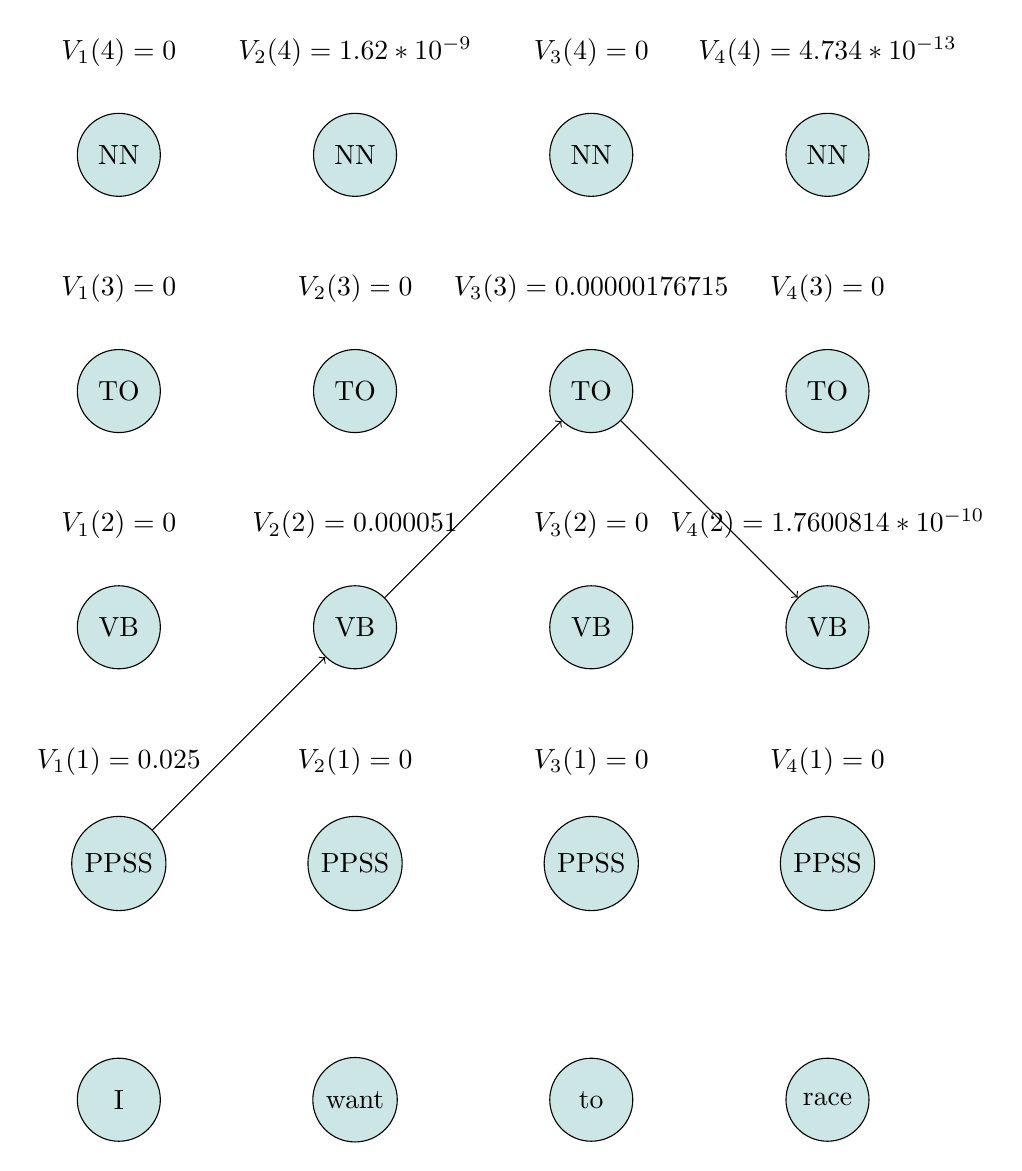
\begin{tikzpicture}[scale=3]

    \node[input] (nn1) at (0,4) {NN};
    \node[above=1cm] at (nn1) {$V_1(4) = 0$};
    \node[input] (nn2) at (1,4) {NN};
    \node[above=1cm] at (nn2) {$V_2(4) = 1.62*10^{-9}$};
    \node[input] (nn3) at (2,4) {NN};
    \node[above=1cm] at (nn3) {$V_3(4) = 0$};
    \node[input] (nn4) at (3,4) {NN};
    \node[above=1cm] at (nn4) {$V_4(4) = 4.734*10^{-13}$};
    
    \node[input] (to1) at (0,3) {TO};
    \node[above=1cm] at (to1) {$V_1(3) = 0$};
    \node[input] (to2) at (1,3) {TO};
    \node[above=1cm] at (to2) {$V_2(3) = 0$};
    \node[input] (to3) at (2,3) {TO};
    \node[above=1cm] at (to3) {$V_3(3) = 0.00000176715$};
    \node[input] (to4) at (3,3) {TO};
    \node[above=1cm] at (to4) {$V_4(3) = 0$};
    
    \node[input] (vb1) at (0,2) {VB};
    \node[above=1cm] at (vb1) {$V_1(2) = 0$};
    \node[input] (vb2) at (1,2) {VB};
    \node[above=1cm] at (vb2) {$V_2(2) = 0.000051$};
    \node[input] (vb3) at (2,2) {VB};
    \node[above=1cm] at (vb3) {$V_3(2) = 0$};
    \node[input] (vb4) at (3,2) {VB};
    \node[above=1cm] at (vb4) {$V_4(2) = 1.7600814*10^{-10}$};

    \node[input] (ppss1) at (0,1) {PPSS};
    \node[above=1cm] at (ppss1) {$V_1(1) = 0.025$};
    \node[input] (ppss2) at (1,1) {PPSS};
    \node[above=1cm] at (ppss2) {$V_2(1) = 0$};
    \node[input] (ppss3) at (2,1) {PPSS};
    \node[above=1cm] at (ppss3) {$V_3(1) = 0$};
    \node[input] (ppss4) at (3,1) {PPSS};
    \node[above=1cm] at (ppss4) {$V_4(1) = 0$};

    \node[input] (x1) at (0,0){I};
    \node[input] (x1) at (1,0){want};
    \node[input] (x1) at (2,0){to};
    \node[input] (x1) at (3,0){race};    
    
    
    \draw[->] (ppss1) -- (vb2);
    \draw[->] (vb2) -- (to3);
    \draw[->] (to3) -- (vb4);
   % \node[input] (x2) at (-3,4){$x_2$}; 

	% inputs of h1
    %\foreach \h [count=\hi ] in {$x_2$,$x_1$,$1$}{
   % 	\node[input] (f1\hi) at (0,\hi*2cm +4cm) {\h};
   % }
    % inputs of h2
   % \foreach \h [count=\hi ] in {$x_2$,$x_1$,$1$}{
   % 	\node[input] (f2\hi) at (0,\hi*2cm -2cm) {\h};
   % }
   
\end{tikzpicture}
\caption{Showing path for question 2}
\label{fig2}
\end{figure}

\section{Question 3}
\begin{enumerate}[leftmargin=\labelsep]
\item[3.1]
\end{enumerate}

\section{Question 4}
\begin{enumerate}[leftmargin=\labelsep]
\item[4.1]
\end{enumerate}

\section{Question 5}
\begin{enumerate}[leftmargin=\labelsep]
\item[5.1]
\end{enumerate}
\end{document}
